\section{Kubernetes Fundamentals}


Kubernetes is an open-source orchestrator for deploying containerized
applications. It was initially developed by Google, inspired by a decade of
experience deploying scalable, reliable systems in containers via
application-oriented APIs. Since its introduction in 2014, Kubernetes has grown
to be one of the world's largest and most popular open-source projects. It has
become the standard API for building cloud-native applications in nearly every
public cloud. Kubernetes is a proven distributed system infrastructure suitable
for cloud-native developers of all scales. It provides the software necessary to
build and deploy reliable, scalable distributed systems.

\begin{figure}
	\centering
	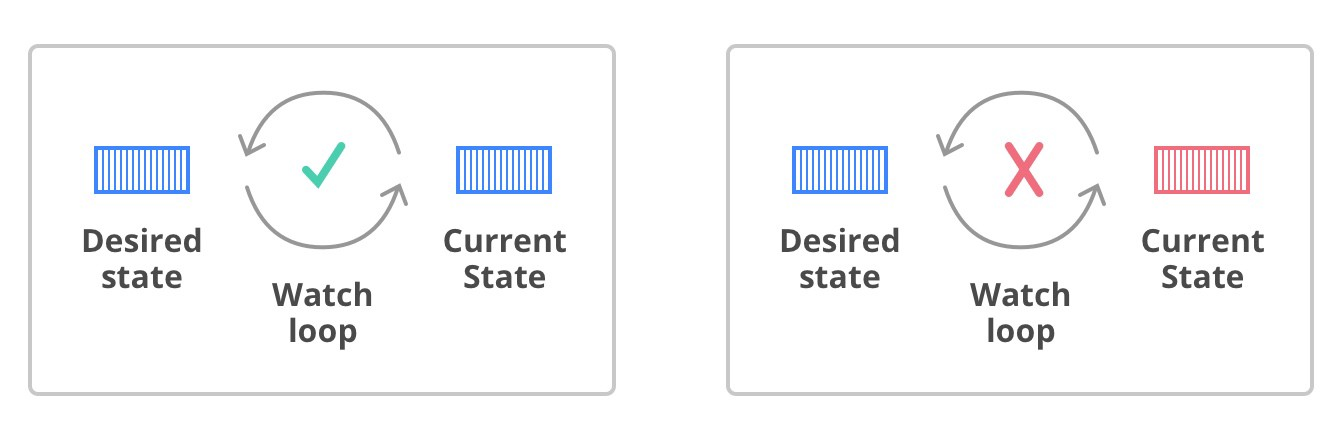
\includegraphics[width=0.8\textwidth]{resources/declarative.jpg}
	\caption{The Kubernetes reconciliation loop}
	% TODO: Replace scheme with the one from vkoukis
\end{figure}

Kubernetes makes application lifecycle management for container-based
applications much more effortless for DevOps via a declarative desired
state-based management approach. It exposes a powerful declarative API that
developers can use to describe the desired state of an application in terms of
Pods, Services, etc., and Kubernetes controllers will take immediate actions to
bring the observed state of the system to the desired state.

\subsection{Kubernetes Architecture}
A Kubernetes cluster consists of a set of worker machines, called nodes, that
run containerized applications. Every cluster has at least one worker node. The
worker nodes host the Pods, which are the components of the application
workload. The control plane manages the worker nodes and the Pods in the
cluster. In production environments, the control plane usually runs across
multiple computers, and a cluster usually runs multiple nodes, providing fault
tolerance and high availability.

\begin{figure}
	\centering
	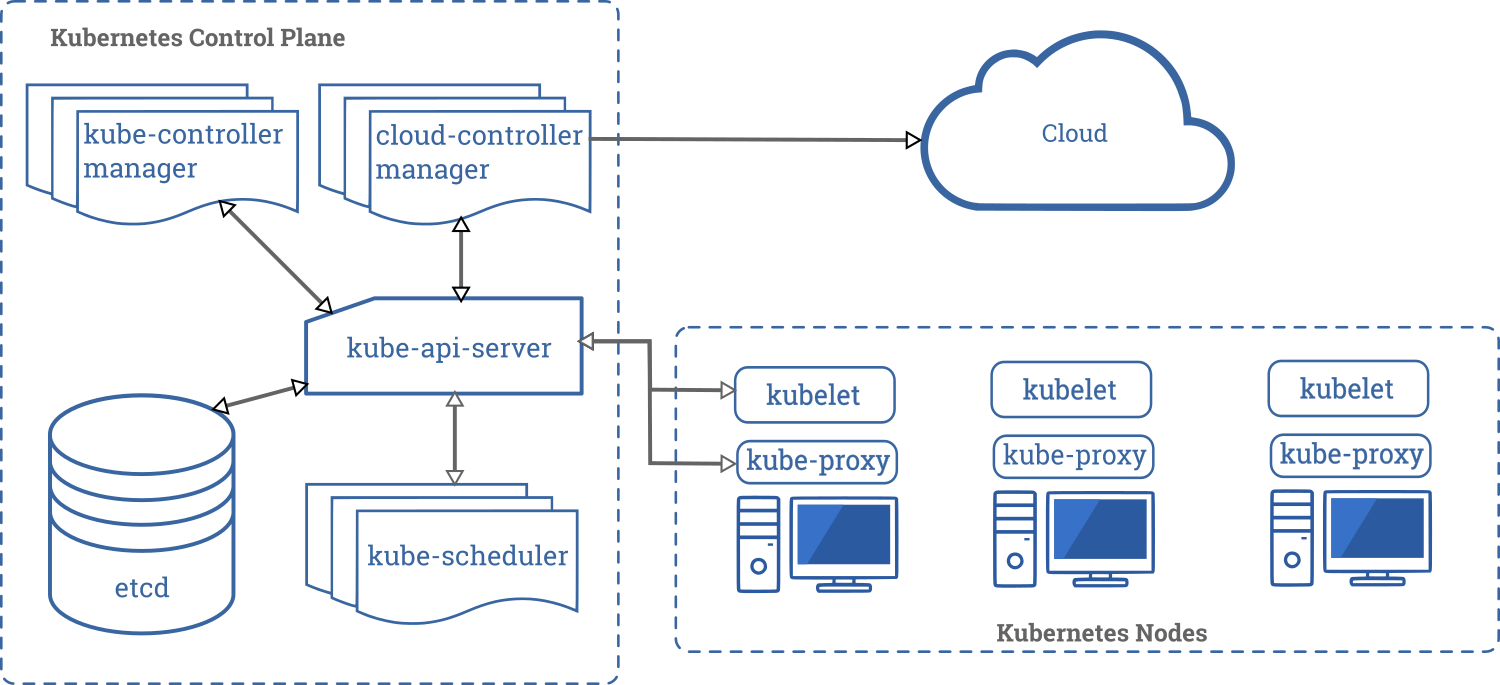
\includegraphics[width=\textwidth]{resources/components-of-kubernetes.png}
	\caption{Kubernetes Architecture}
\end{figure}


\subsection{Kubernetes Control Plane Components}
The control plane's components make global decisions about the cluster (for
example, scheduling), as well as detecting and responding to cluster events (for
example, starting up a new Pod when a deployment's replicas field is
unsatisfied).

The main control plain components are:

\begin{itemize}
	\item
	      \texttt{kube-apiserver}: The API server is a component of the
	      Kubernetes control plane that exposes the Kubernetes API. The API
	      server is the front end of the Kubernetes control plane. The primary
	      implementation of a Kubernetes API server is \co{kube-apiserver}.
	      \co{Kube-apiserver} is designed to scale horizontally, i.e., it scales
	      by deploying more instances. A cluster may run several instances of
	      \co{kube-apiserver} and balance traffic between those instances.
	\item
	      \texttt{etcd}: A consistent and highly-available key-value store that
	      is used as Kubernetes' backing store for all cluster data. Distributed
	      and fault-tolerant, etcd is an open-source, key-value store database
	      that stores configuration data and information about the state of the
	      cluster. Etcd may be configured externally, although it is often part
	      of the Kubernetes control plane.

	      Etcd stores the cluster state based on the Raft consensus algorithm.
	      This helps cope with a common problem in the context of replicated
	      state machines and involves multiple servers agreeing on values. Raft
	      defines three different roles: leader, candidate, and follower, and
	      achieves consensus by electing a leader.

	      In this way, etcd acts as the single source of truth (SSOT) for all
	      Kubernetes cluster components, responding to queries from the control
	      plane and retrieving various parameters of the state of the
	      containers, nodes, and Pods and other cluster components, in general.


	\item
	      \texttt{kube-scheduler}: Control plane component that watches for
	      newly created Pods with no assigned node and selects a node for them
	      to run on. Factors considered for scheduling decisions include
	      individual and collective resource requirements,
	      hardware/software/policy constraints, affinity, and anti-affinity
	      specifications, data locality, inter-workload interference, and
	      deadlines.
	\item
	      \texttt{kube-controller-manager}: Control plane component that runs
	      controller processes. Logically, each controller is a separate
	      process, but to reduce complexity, they are all compiled into a single
	      binary and run in a single process. Some types of these controllers
	      are:
	      \begin{itemize}
		      \tightlist
		      \item
		            \textbf{Node controller}: Responsible for noticing and
		            responding when nodes go down.
		      \item
		            \textbf{Job controller}: Watches for \co{Job} objects that
		            represent one-off tasks, then creates Pods to run those
		            tasks to completion.
		      \item
		            \textbf{Endpoints controller}: Populates the Endpoints
		            object (that is, joins Services \& Pods).
		      \item
		            \textbf{Service Account} \& \tbf{Token controllers}: Create
		            default accounts and API access tokens for new namespaces.
	      \end{itemize}
	\item
	      \texttt{cloud-controller-manager}: Kubernetes control plane component
	      that embeds cloud-specific control logic. The cloud controller manager
	      lets a user link their cluster into their cloud provider's API, and
	      separates out the components that interact with that cloud platform
	      from components that only interact with their cluster. The
	      cloud-controller-manager only runs controllers that are specific to
	      your cloud provider. If a Kubernetes cluster runs on a user's
	      premises, the cluster does not have a cloud controller manager.
\end{itemize}

\subsection{Kubernetes Node Components}

Node components run on every node, maintaining running Pods and providing the
Kubernetes runtime environment.

Every node runs the following components:

\begin{itemize}
	\item
	      \texttt{kubelet}: An agent that makes sure that containers are running
	      in a Pod.
	\item
	      \texttt{kube-proxy}: kube-proxy is a network proxy implementing part
	      of the Kubernetes Service concept. Kube-proxy maintains network rules
	      on nodes. These network rules allow network communication to the
	      user's Pods from network sessions inside or outside of their cluster.
	      Kube-proxy uses the operating system packet filtering layer if there
	      is one and it's available. Otherwise, kube-proxy forwards the traffic
	      itself.
	\item
	      \texttt{Container Runtime}: The container runtime is the software that
	      is responsible for running containers. Kubernetes supports container
	      runtimes such as containerd, CRI-O, and any other implementation of
	      the Kubernetes CRI (Container Runtime Interface).
\end{itemize}

\subsection{The Kubernetes API}

The core of Kubernetes' control plane is the API server. The API server exposes
an HTTP API that lets end-users, different cluster parts, and external
components communicate. The Kubernetes API lets the user query and manipulate
the state of API objects in Kubernetes (for example, Pods, Namespaces,
ConfigMaps, and Events). Kubernetes generally leverages common RESTful
terminology to describe the API concepts:


\begin{itemize}
	\tightlist
	\item A \textit{resource type} is the name used in the URL (Pods,
	      Namespaces, Services).
	\item All resource types have a concrete representation (their object
	      schema) which is called a \textit{kind}.
	\item A list of instances of a resource is known as a \textit{collection}.
	\item A single instance of a resource type is called a resource and usually
	      represents an object.
\end{itemize}

Almost all object resource types support the standard HTTP verbs - \texttt{GET},
\texttt{POST}, \texttt{PUT}, \texttt{PATCH}, and \texttt{DELETE}. Kubernetes
also uses its own, often written lowercase, to distinguish them from HTTP verbs.
Kubernetes uses the term ``list'' to describe returning a collection of
resources to distinguish from retrieving a single resource, usually called a
``get''. All resource types are scoped either to the cluster or to a
\textit{namespace}. A namespace-scoped resource type will be deleted when its
namespace is deleted, and access to that resource type is controlled by
authorization checks on the namespace scope.

\subsection{Kubernetes Objects}

Kubernetes \textit{objects} are persistent entities in the Kubernetes system.
Kubernetes uses these entities to represent the state of the cluster.
Specifically, they can describe:
\begin{itemize}
	\tightlist
	\item What containerized applications are running and on which nodes.
	\item The resources available to those applications.
	\item The policies around how those applications behave, such as restart
	      policies, upgrades, and fault-tolerance.
\end{itemize}

A Kubernetes object is a ``record of intent''; once a user creates the object,
the Kubernetes system will constantly work to ensure that the object exists. By
creating an object, a user is effectively telling the Kubernetes system what
they want their cluster's workload to look like.

%TODO: Add about put update delete patch
%https://kubernetes.io/docs/reference/using-api/api-concepts/

\subsubsection{The \co{Pod} Object}\label{background:Pod}

Pods  are the smallest deployable artifact in a Kubernetes cluster. A
\textit{Pod} represents a collection of application containers and volumes
running in the same execution environment. This means all of the containers in a
Pod always land on the same machine. Each container within a Pod runs in its own
cgroup, but they share several Linux namespaces. Applications running in the
same Pod share the same IP address and port space (network namespace), have the
same hostname (UTS namespace), and can communicate using native interprocess
communication channels over System V IPC or POSIX message queues (IPC
namespace). However, applications in different Pods are isolated from each
other; they have different IP addresses, different hostnames, etc. Containers in
different Pods running on the same node might also be on different servers.

\begin{figure}[ht]
	\centering
	\includegraphics[width=0.8\textwidth]{resources/Pod-lifecycle.png}
	\caption{The lifecycle of a Pod}
	% TODO: PDF
\end{figure}

\paragraph*{Phase}
The \textit{phase} of a Pod is a simple, high-level summary of where the Pod is
in its lifecycle. Each Pod follows a defined lifecycle, starting in the
\co{Pending} phase, moving through \texttt{Running} if at least one of its
primary containers starts OK, and then through either the \texttt{Succeeded} or
\texttt{Failed} phases depending on whether any container in the Pod terminated
in failure.

More specifically, the phase of a Pod can be:

\begin{itemize}
	\tightlist
	\item
	      \texttt{Pending}: the Pod has been accepted by the system, but one or
	      more of the containers has not been started. This includes time before
	      being bound to a node, as well as time spent pulling images onto the
	      host.
	\item
	      \texttt{Running}: the Pod has been bound to a node and all of the
	      containers have been started. At least one container is still running
	      or is in the process of being restarted.
	\item
	      \text	{Succeeded}: all the containers of the Pod have voluntarily
	      terminated with a container exit code of 0, and the system is not
	      going to restart any of these containers.
	\item
	      \texttt{Failed}: all the containers of the Pod have terminated, and at
	      least one container has terminated in a failure (exited with a
	      non-zero exit code or was stopped by the system).
	\item
	      \texttt{Unknown}: for some reason the state of the Pod could not be
	      obtained, typically due to an error in communicating with the host of
	      the Pod.
\end{itemize}

\paragraph*{Status}
\label{section:unschedulable-Pod}
A Pod has a \texttt{PodStatus}, which has an array of \texttt{PodConditions}
through which the Pod has or has not passed:
\begin{itemize}
	\tightlist
	\item \co{PodScheduled}: the Pod has been scheduled to a node.
	\item \co{ContainersReady}: all containers in the Pod are ready.
	\item \co{Initialized}: all init containers have completed successfully.
	\item \co{Ready}: the Pod is able to serve requests and should be added to
	      the load balancing pools of all matching Services.
\end{itemize}

\paragraph*{Unschedulable Pods}
\label{section:Pod-unschedulable}

The cluster scheduler is responsible for assigning a node for the Pod to run on.
It assigns a node by setting the \co{spec.nodeName} field of the Pod. If the
scheduler fails to find a place to run the Pod, it sets \co{PodScheduled}
\co{PodCondition} to \co{False} and reason to \co{Unschedulable}. An
unschedulable Pod will remain in \co{Pending} phase.

In the context of this thesis, we will refer to a Pod that could not be
scheduled  as ``\textit{unschedulable Pod}'' or, equivalently, ``\textit{Pending
Pod}''.
\paragraph*{Resource requests and limits}
\label{section:pod-requests}

Compute resources are measurable quantities that can be requested, allocated,
and consumed. For instance, but not limited to, CPU and memory are some types of
computing resources.

The user can specify resource requests and limits for each container of the Pod.
The scheduler uses the requests to decide which node assign to the Pod. The
kubelet uses the limits for a container and enforces them so that the running
container cannot use more of that resource than the limit a user has set. The
kubelet also reserves at least the requested amount of that system resource
specifically for that container to use. If the node where a Pod is running has
enough of that resources available, it is possible (and allowed) for a container
to use more than requested. However, a container cannot use more than the limit
of that resource.

\lstinputlisting[label={listing:pod-requests},language=yaml,caption={Requests and limits of a Pod's container}]{code/pod-requests.yaml}

\subsubsection{The \co{Node} Object}
Kubernetes runs the workload by placing Pods to run on nodes. Depending on the
cluster, a node may be a virtual or physical machine. The control plane manages
each node and contains the services necessary to run Pods. A node registered in
the Kubernetes cluster is represented using a \co{Node} object on the API
Server.

\paragraph*{Node taints}
Taints and tolerations are a mechanism that users can use to ensure that Pods
are not placed on inappropriate nodes. Taints are added to nodes, while
tolerations are defined in the Pod specification. A node can have one or many
taints associated with it. When a user taints a node, it repells all the Pods
except those that have a toleration for that taint.

% TODO: define in or define on

A taint can produce three possible effects:
\begin{itemize}
	\tightlist
	\item \co{NoSchedule}: The scheduler will only allow scheduling
	      Pods that have tolerations for the tainted nodes.
	\item \co{PreferNoSchedule}: The scheduler will try to avoid
	      scheduling Pods that don’t have tolerations for the tainted nodes.
	\item \co{NoExecute}: Kubernetes will evict the running Pods from the nodes
	      if the Pods don’t have tolerations for the tainted nodes.
\end{itemize}

\paragraph*{Node status}
\label{section:node-status}
Each \co{Node} object has a \texttt{/status} subresource that indicates the status of
the node. The status contains multiple conditions for the node and is managed by
the node controller. Some conditions that are often encountered include:

\begin{itemize}
	\tightlist
	\item \co{MemoryPressure}: If \co{True}, it indicates that the node is
	      running out of memory.
	\item \co{DiskPressure}: A \co{True} value in this field indicates that the
	      node lacks enough space.
	\item \co{PIDPressure}: If too many processes are running on the node, this
	      field will be \co{True}.
	\item \co{NetworkUnavailable}: If the network for the node is not correctly
	      configured, this will be \co{True}.
	\item \co{Ready}: If the node is healthy and ready to accept Pods, this will
	      be \co{True}. In this field, a \co{False} is equivalent to the
	      \texttt{NotReady} status in the get nodes output. It can also have the
	      Unknown value, which means the node controller has not heard from the
	      node in the last \texttt{node-monitor-grace-period}.
\end{itemize}

In the context of the Cluster Autoscaler and the Scheduler, a node will be
considered as ``\textit{Unready}''  if:
\begin{itemize}
	\tightlist
	\item It has \co{Pod.spec.unschedulable} field. This field indicates the
	      node shall not accept Pods.
	\item The \co{Node} object does not have any condition of type \co{Ready}.
	\item A condition of type \co{Ready} exists and the its status is
	      \co{False}.
	\item A condition of type \co{DiskPressure} or \co{PIDPressure} or
	      \co{NetworkUnavailable} with its corresponding status set to
	      \co{True}. exists.
\end{itemize}

The rest of the nodes shall be considered as \texttt{Ready}.

A node that cannot accept Pods will be referred to as ``\textit{unschedulable}''
node.

\paragraph*{Node allocatable}
\label{section:node-allocatable}

\textit{Allocatable} on a Kubernetes node is defined as the amount of computing
resources that are available for Pods.  The total resources (capacity) of a node
are categorized into:

\begin{itemize}
	\item \co{kube-reserved}: resource reservation for kubernetes system daemons
	      like the kubelet, container runtime, node problem detector, etc. It is
	      not meant to reserve resources for system daemons that are run as
	      Pods.
	\item \co{system-reserved}: resource reservation for OS system daemons like
	      sshd, udev, etc. system-reserved should reserve memory for the kernel
	      too since kernel memory is not accounted to Pods in Kubernetes at this
	      time.
	\item \co{eviction-threshold}: specifies limits that trigger evictions when
	      node resources drop below the reserved value.
	\item \co{allocatable}: the remaining node resources available for
	      scheduling of Pods.
\end{itemize}

\begin{figure}
	\centering
	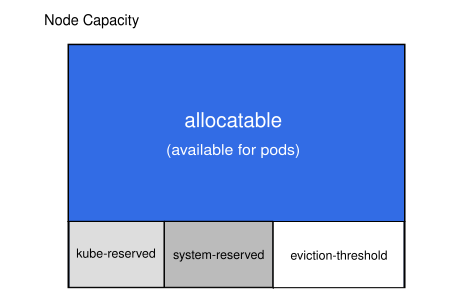
\includegraphics[width=0.7\textwidth]{resources/node-capacity.png}
	\captionof{figure}{Node resources: capacity and allocatable}
	\label{fig:test1}
\end{figure}

\subsubsection{The \co{PodDisruptionBudget} Object}
\label{section:Pod-disruption-budge}

Pods do not disappear until someone (a person or a controller) destroys them or
there is an unavoidable hardware or system software error.

The unavoidable cases are called \emph{involuntary disruptions} and include:
\begin{itemize}
	\tightlist
	\item A hardware failure of the physical machine backing the node.
	\item Cluster administrator deletes VM (instance) by mistake.
	\item Cloud provider or hypervisor failure makes VM disappear.
	\item A kernel panic.
	\item The node disappears from the cluster due to cluster network partition.
	\item Eviction of a Pod due to the node being out-of-resources.
\end{itemize}

All other cases are called \emph{voluntary disruptions}. These include both
actions initiated by the application owner and those initiated by a Cluster
Administrator. Typical voluntary disruptions include:

\begin{itemize}
	\tightlist
	\item Deleting the deployment or other controller that manages the Pod.
	\item Updating a deployment's Pod template causing a restart.
	\item Directly deleting a Pod.
	\item Draining a node for repair or upgrade.
	\item Draining a node from a cluster to scale the cluster down.
	\item Removing a Pod from a node to permit something else to fit on that
	      node.
\end{itemize}

A \texttt{PodDisruptionBudget} (PDB) limits the number of Pods of a replicated
application that are down simultaneously from voluntary disruptions. For
example, a web front end might want to ensure that the number of replicas
serving load never falls below a certain percentage of the total.

A PDB specifies the number of replicas that an application can tolerate having,
relative to how many it is intended to have. For example, a Deployment that has
a \texttt{.spec.replicas:\ 5} is supposed to have 5 Pods at any given time. If
its PDB allows for there to be 4 at a time, then the Eviction API will allow
voluntary disruption of one (but not two) Pods at a time.

Involuntary disruptions cannot be prevented by PDBs; however they do count
against the budget. Pods which are deleted or unavailable due to a rolling
upgrade to an application do count against the disruption budget.

\subsubsection{The \co{Deployment} Object}
\label{section:deployment}
A \co{Deployment} resource ensures that a specified number of Pod
\textit{replicas} are running at any time. In other words, a Deployment ensures
that a Pod or homogeneous set of Pods are always up and available. If there are
too many Pods, it will kill some. If there are too few, the Deployment will
start more.

\subsubsection{The \co{DaemonSet} Object}
\label{section:daemone-set}

A \co{DaemonSet} (DS) resource ensures that all Nodes run a copy of a Pod. As
nodes are added to the cluster, Pods are added to them. As nodes are removed
from the cluster, those Pods are garbage collected. Deleting a DaemonSet will
clean up the Pods it created.

\subsubsection{The \co{PersistentVolumeClaim} object}

A \co{PersistentVolumeClaim} (PVC, or equivalently referred to as ``claim'')) is
a request for storage by a user. Claims can request specific size and access
modes, e.g., they can be mounted \co{ReadWriteOnce}, \co{ReadOnlyMany} or
\co{ReadWriteMany}, etc.


\paragraph*{Phase}
The \textit{Phase} of a PVC can be one of the following:
\label{section:pvc-phase}
\begin{enumerate}
	\tightlist
	\item \texttt{Pending}: the PVC is not yet bound.
	\item \texttt{Bound}: the PVC is bound to a PV.
	\item \texttt{Lost}: the PVC lost its underlying PV. The claim was bound to
	      a  PV and this volume does not exist any longer and all data on it was
	      lost.
\end{enumerate}


\subsubsection{The \co{PersistentVolume} object}

A \co{PersistentVolume} (PV, or equivalently referred to as ``volume'') is a
piece of storage in the cluster that has been provisioned by an administrator or
dynamically provisioned using Storage Classes. It is a resource in the cluster.
PVs have a lifecycle independent of any individual Pod that uses the PV. This
\co{API} object captures the details of the implementation of the storage, be that
NFS, iSCSI, or a cloud-provider-specific storage system.

\begin{figure}[ht]
	\centering
	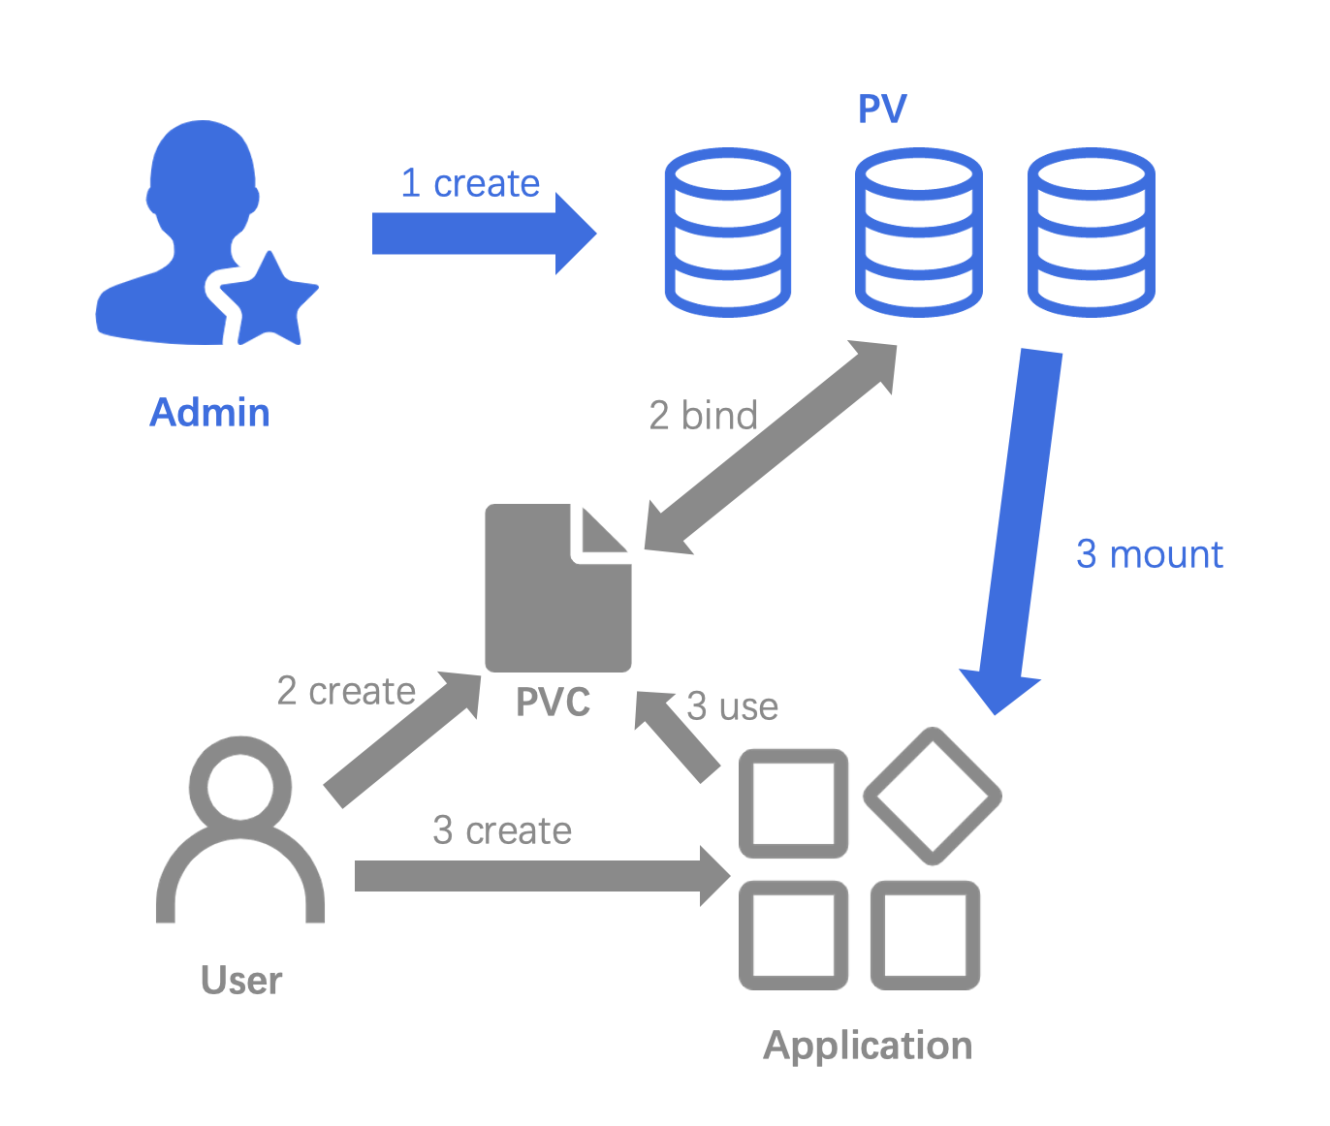
\includegraphics[width=0.6\textwidth]{resources/pvc-lifecycle.png}
	\caption{The lifecycle of a PVC and PV in the case of static provisioning}
\end{figure}

\paragraph*{Phase} A PV can be in one of the following phases:
\label{section:pv-phase}
\begin{itemize}
	\tightlist
	\item \texttt{Available}: the PV is not yet bound; it is available to be
	      matched to a PVC.
	\item \texttt{Bound}: the PV is bound to a PVC.
	\item \texttt{Released}: the PVs must be recycled before becoming available
	      again. This phase is used by the persistent volume claim binder to
	      signal to another process to reclaim the resource.
	\item \texttt{Failed}: the PV has failed to be correctly recycled or deleted
	      after being released from a claim.
\end{itemize}


\paragraph*{Binding}
PVCs are requests for storage resources; each PVC gets bound to a PV that
matches the PVC's requested storage amount and access modes. Each PV gets bound
to one PVC only, and vice versa. The binding between them is bidirectional.  A
PV will remain unbound till it is matched to a PVC. The binding is illustrated
in Figure \ref{figure:pvc-pv}.

\begin{figure}[ht]
	\centering
	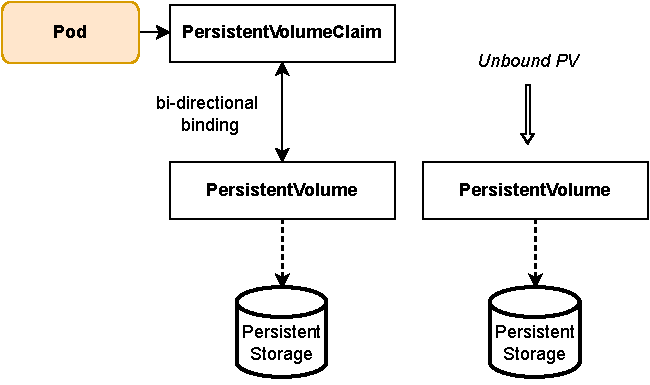
\includegraphics[width=0.8\textwidth]{resources/pvc-pv-binding.pdf}
	\caption{A Pod requests a volume using a PVC and the PVC gets bound to a PV. The PV object stores the details for the underlying persistent storage piece.}
	\label{figure:pvc-pv}
\end{figure}

The interaction between PVs and PVCs follows this lifecycle:
\begin{enumerate}
	\item \textbf{Provisioning}: There are two ways PVs may be provisioned:
	      statically or dynamically.
	      \begin{itemize}
		      \item \textbf{Statically}: A cluster administrator creates some
		            PVs. They carry the details of the actual storage, which is
		            available for use by cluster users. They exist in the
		            Kubernetes API and are available for consumption. \item
		            \textbf{Dynamically}: When none of the static PVs the
		      \item \textbf{Dynamically}: When none of the static PVs the
		            administrator created matches a user's
		            PersistentVolumeClaim, the storage system may try to
		            dynamically provision a volume for the PVC. This
		            provisioning relies on storage classes: the PVC must request
		            a storage class, and the administrator must have created and
		            configured that class for dynamic provisioning. Claims that
		            do not specify a storage class effectively disable dynamic
		            provisioning for themselves.
	      \end{itemize}
	\item \textbf{Binding}: A user creates a PersistentVolumeClaim with a
	      specific amount of storage requested and with certain access modes. A
	      control loop (the PersistentVolumeController) in the Kubernetes
	      control plane watches for new PVCs, finds a matching PV (if possible),
	      and binds them together. If a PV was dynamically provisioned for a new
	      PVC, the loop binds that PV to the PVC. Otherwise, the user will get
	      at least what they asked for, but the volume may be more than what was
	      requested. Once bound, PersistentVolumeClaim binds are exclusive,
	      regardless of how they were bound. A PVC to PV binding is a one-to-one
	      mapping, using a \co{ClaimRef} which is a bidirectional binding
	      between the PersistentVolume and the PersistentVolumeClaim. Claims
	      will remain unbound indefinitely if a matching volume does not exist.
	      Claims will be bound as matching volumes become available. For
	      example, a cluster provisioned with many 50Gi PVs would not match a
	      PVC requesting 100Gi. The PVC can be bound when a 100Gi PV is added to
	      the cluster.
	\item \textbf{Using}: Pods use claims as volumes. The cluster inspects the
	      claim to find the bound volume and mounts that volume for a Pod. For
	      volumes that support multiple access modes, the user specifies which
	      mode is desired when using their claim as a volume in a Pod. Once a
	      user has a claim and that claim is bound, the bound PV belongs to the
	      user for as long as they need it. Users access their claimed PVs by
	      including a \co{persistentVolumeClaim} section in a Pod's \co{volumes}
	      block.
\end{enumerate}

In the context of this thesis, a PVC will be also referred to as a
``\texttt{claim}''

\paragraph*{Node affinity}
\label{section:background-pv-node-affinity}

A PV can specify node affinity to define constraints that limit what nodes this
volume can be accessed from. The \co{nodeAffinity} field of the PV is a label
selector that matches nodes with the appropriate labels. Labels are key/value
pairs that are attached to objects.

The node affinity of a PV is used in the following way to indicate a volume is
local to a node:
\begin{enumerate}
	\tightlist
	\item The storage driver sets on each \texttt{Node} object a unique label.
	\item The storage driver sets the corresponding node affinity of the PV to
	      match only the unique label of the node.
\end{enumerate}

Listing ~\ref{listing:pv-affinity} presents a PV with node affinity that matches
node having the label \co{node:node-1}.

\lstinputlisting[label={listing:pv-affinity},language=yaml,caption={A PV with node affinity}]{code/node-affinity.yaml}

\subsubsection{The \co{StorageClass} Object}

A \co{StorageClass} is a Kubernetes resource that enables dynamic storage
provisioning. A StorageClass provides a way for administrators to describe the
``classes'' of storage they offer. The administrator configures the
StorageClass, which can then no longer be modified.

A storage class can specify a \co{volumeBindingMode}, which is either
\co{Immediate} or \co{WaitForFirstConsumer}:
\begin{itemize}
	\item  \co{Immediate}: Indicates that volume binding and dynamic
	      provisioning occur once the user creates the PersistentVolumeClaim.
	      For storage backends that are topology-constrained and not globally
	      accessible from all nodes in the cluster, PersistentVolumes will be
	      bound or provisioned without knowledge of the Pod's scheduling
	      requirements, possibly resulting in unschedulable Pods.
	\item \co{WaitForFirstConsumer}: The binding and provisioning of a
	      PersistentVolume will be delayed until a Pod using the
	      PersistentVolumeClaim is created. PersistentVolumes will be selected
	      or provisioned conforming to the topology that is specified by the
	      Pod's scheduling constraints.
\end{itemize}


\subsection{The Eviction API}
\label{section:background-eviction}

When deleting a resource on Kubernetes, the API server will put a
\co{deletionTimestamp} on the resource object. Unless there are any finalizers
on the object, the object will be removed from the API Server.

In the case of Pods, apart from the classic \co{DELETE} operation, Kubernetes
offers an extra API to initiate the deletion of the Pod: the \co{Eviction} API.
The main difference with the delete operation is that API-initiated evictions
respect the configured PodDisruptionBudgets and
\co{terminationGracePeriodSeconds}. So, if a user tries to \textit{evict} a Pod
and the corresponding PodDisruptionBudget does not allow the disruption of the
Pod, the Pod will not be deleted. Instead, issuing a classical \co{DELETE}
operation will remove the Pod, no matter what the PodDisruptionBudget specifies.

\subsection{The Cordon \& Drain Operations}
\label{section:cordon-drain}

The Kubernetes command-line tool, \co{kubectl}, allows a user to run commands
against Kubernetes clusters. The tool allows the complete management of the
cluster. Two essential operations used for the maintenance of the cluster are
the \textit{cordon} and the \textit{drain} operations.

\paragraph*{Cordon operation}
\textit{Cordon} is an operation offered by the \co{kubectl} CLI tool that marks
the node as \textit{unschedulable}. Marking a node as unschedulable prevents the
scheduler from placing new Pods onto that node but does not affect existing Pods
running on it. This is a preparatory step before a node reboot or other
maintenance.

The admin of the cluster can execute the cordon operation by running \co{kubectl
	cordon}. When cordoning a node, the tool adds the \textit{unschedulable
	taint} \footnote{Unschedulable taint:
	\co{node.kubernetes.io/unschedulable:NoSchedule}} on the node and also sets
	the \co{nodes.spec.unschedulable} field to \co{True}.

We will refer to the action of marking the node as unschedulable as
``\textit{cordoning the node}'' and the node as ``\textit{cordoned}''.

\paragraph*{Drain operation}

The \textit{drain} operation is used to remove workload from a node. It is run
in case the node needs maintenance, or it needs to be removed from a cluster.
The drain operation cordons the node to mark it as unschedulable, and evicts all
the Pods from the node.  Evictions allow the Pod's containers to terminate
gracefully and will respect the PodDisruptionBudgets the user has specified.

The admin of the cluster can execute the drain operation by running \co{kubectl
	drain}. If \co{kubectl drain} returns successfully, it indicates that all
	the Pods have been safely evicted (respecting the desired graceful
	termination period and the PodDisruptionBudget that is defined). It is then
	safe to bring down the node by powering down its physical machine or
	deleting its virtual machine if it runs on a cloud platform.

\section{Kubernetes Controllers}
In Kubernetes, controllers are control loops that watch the state of the
cluster, then make or request changes where needed. Each controller tries to
move the current cluster state closer to the desired state. A controller tracks
at least one Kubernetes resource type. These objects have a \co{spec} field
representing the desired state. The controllers for that resource are
responsible for making the current state come closer to that desired state.

In this section, we will describe some of the controller that play a significant
role in the storage system of Kubernetes.


\subsection{The PersistentVolume Controller}

The \co{PersistentVolumeController} is a controller that synchronizes
PersistentVolumeClaims and PersistentVolumes.  It binds PVs and PVCs and manages
their lifecycles. If the PVC references a StorageClass with static provisioning,
the control loop attempts to find a matching PV and then binds it to the PVC. In
the case of dynamic provisioning, as soon as the PV gets provisioned for the
PVC, the control loop binds them together.

\subsection{The AttachDetach Controller}

The \co{AttachDetach} controller manages volume attach and detach operations. It
looks for any Pods that get scheduled on a node and triggers the attach
operation, i.e., it creates a \co{VolumeAttachment} object to signal the
external attacher that it shall issue a \co{ControllerPublish} call to the CSI
driver. Similarly, when no Pods use a volume on a node, the controller executes
a detach operation: deletes the \co{VolumeAttachment} object to signal the external
attacher it shall issue a \co{ControllerUnpublish} request to the CSI driver.


\subsection{Kubernetes Admission Controllers}

An \textit{admission controller} is a piece of code that intercepts requests to
the Kubernetes API server prior to the persistence of the object but after the
request is authenticated and authorized. Admission controllers may be
\textit{validating}, \textit{mutating}, or both. Mutating controllers may modify
related objects to the requests they admit; validating controllers may not.

The admission control process proceeds in two phases. In the first phase, it
runs the mutating admission controllers. In the second phase, it runs the
validating admission controllers. If any controller in either phase rejects the
request, the entire request is rejected immediately and an error is returned to
the end-user.

Various admission controllers come compiled into the \co{kube-apiserver} binary,
and out of them, there are two controllers of particular interest, the
\co{MutatingAdmissionWebhook} and \co{ValidatingAdmissionWebhook}:
\begin{itemize}
      \tightlist
      \item \co{MutatingAdmissionWebhook}: This admission controller calls any
            mutating webhooks which match the request. Matching webhooks are called
            serially; each one may modify the object if desired.

      \item \co{ValidatingAdmissionWebhook}: This admission controller calls any
            validating webhooks which match the request. Matching webhooks are
            called in parallel; if any of them rejects the request, the request
            fails.
\end{itemize}

The admission controller phases are shown in Figure
~\ref{figure:admission-controller}.
\begin{figure}[ht]
      \centering
      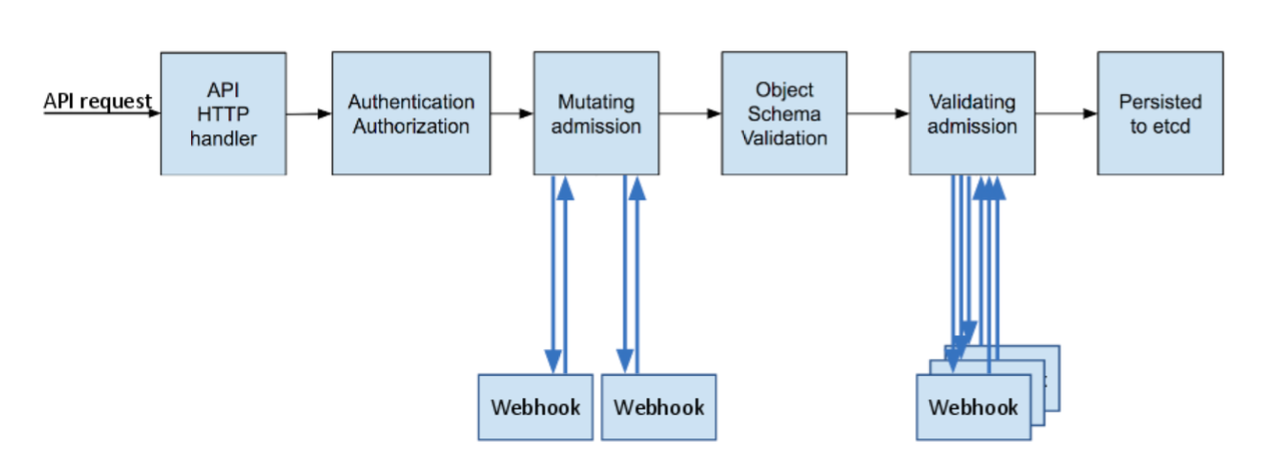
\includegraphics[width=\textwidth]{resources/admission-controller-phases.png}
      \caption{Admission controller phases}
      \label{figure:admission-controller}
\end{figure}

\section{Kubernetes Admission Webhooks}

Admission webhooks are HTTP callbacks that receive admission requests and do
something with them. Two types of admission webhooks can be defined:
\textit{validating admission} webhook and \textit{mutating admission} webhook.

Mutating admission webhooks are invoked first, and can modify objects sent to
the API server to enforce custom defaults. After all object modifications are
complete, and after the incoming object is validated by the API server,
validating admission webhooks are invoked and can reject requests to enforce
custom policies.The admin of the cluster can dynamically configure what
resources are subject to what admission webhooks via
\co{ValidatingWebhookConfiguration} or \co{MutatingWebhookConfiguration} API
objects.

\paragraph*{\co{MutatingWebhookConfiguration} Object}

Each \texttt{MutatingWebhookConfiguration} contains a list of webhooks,
specified at \co{webhooks} field. Each of the webhooks defined, may specify the
following fields:
\begin{itemize}
      \tightlist
      \item \texttt{rules}: A list of rules used to determine if a request to
            the API server should be sent to the webhook. Each rule specifies
            one or more operations, apiGroups, apiVersions, and resources, and a
            resource scope.
      \item  \texttt{failurePolicy}: Defines how unrecognized errors and timeout
            errors from the admission webhook are handled. Allowed values are
            \texttt{Ignore} or \texttt{Fail}.
      \item \texttt{namespaceSelector}:  Defines whether to run the webhook on a
            request for a namespaced resource (or a \texttt{Namespace} object) based
            on whether the namespace labels match the selector. If the object is a
            cluster scoped resource other than a Namespace, \texttt{namespaceSelector}
            has no effect.
\end{itemize}

\section{The Kubernetes Operator Pattern}
\label{section:operator-pattern}

A Kubernetes operator is a custom application-specific controller that extends
the functionality of the Kubernetes API to create, configure, and manage
instances of complex applications on behalf of a Kubernetes user. It builds upon
the fundamental Kubernetes resource and controller concepts but includes domain
or application-specific knowledge to automate the entire life cycle of the
software it manages. It uses \textit{custom resources} to manage applications
and their components. The user within a custom resource provides high-level
configuration and settings. The Kubernetes operator translates the high-level
directives into low-level actions based on best practices embedded within the
operator's logic.

A \co{CustomResourceDefinition} object (CRD) defines a custom resource and lists
out all the configurations available to users of the operator. The Kubernetes
API can handle custom resource definitions just like built-in objects, including
interaction via \co{kubectl} and inclusion in role-based access control (RBAC)
policies.

\begin{figure}[ht]
	\centering
	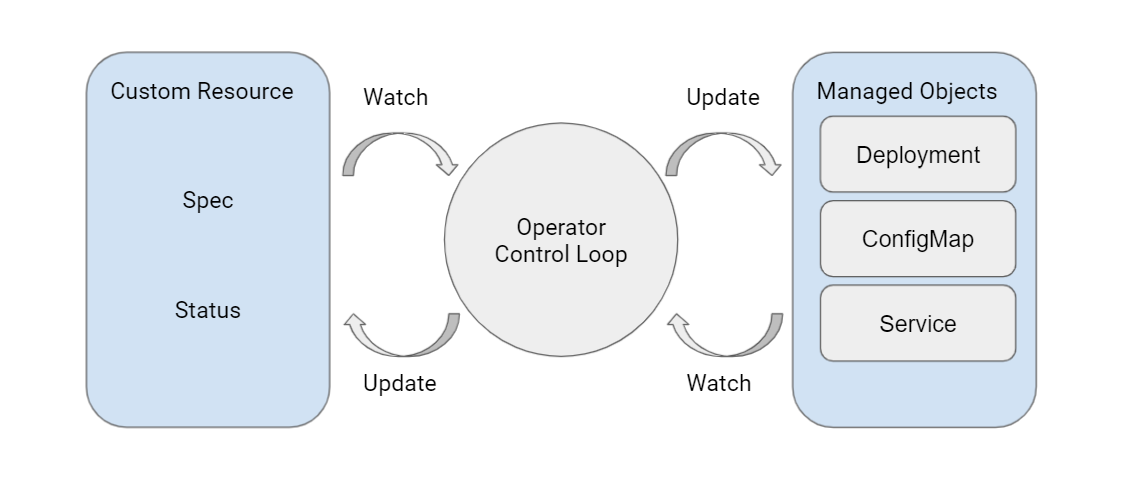
\includegraphics[width=0.8\textwidth]{resources/operator.png}
	\caption{The Kubernetes operator pattern}
\end{figure}
